%-----------------------------------------------------------------------------%
\chapter{\babTiga}
\label{bab:3} 

Bab ini secara umum memaparkan tentang metodologi penelitian yang ditempuh dalam mengembangkan sistem PeerToCP. Lebih lanjut, akan mencakup mengenai pendekatan, rincian tahapan, yang termasuk desain sistem, serta metode evaluasi sistem.

\section{Pendekatan dan Tahapan Penelitian}

\begin{figure}
    \centering
    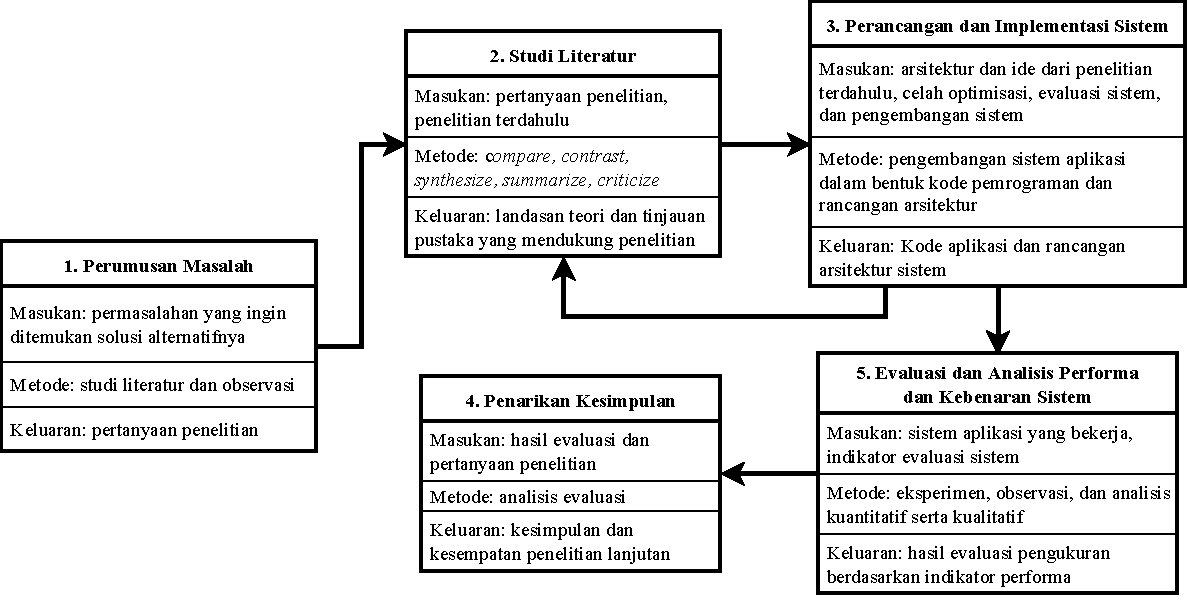
\includegraphics[scale=0.7]{assets/skripsi/MetodePenelitian.pdf}
    \caption{Bagan Alur Penelitian}
    \label{fig:my_label}
\end{figure}

\section{Desain Sistem}

\subsection{Kode dan Kompilasi}

Proses kompilasi merupakan proses mengonversi kode dari bahasa dengan level yang lebih tinggi dan dapat dimengerti oleh manusia menjadi kode biner yang dapat dimengerti oleh mesin. Pada penelitian ini, selain editor kode yang bersifat kolaboratif, proses kompilasi kode tunggal juga hendaknya dapat dilakukan oleh salah satu pengguna. Proses kompilasi ini membutuhkan kompilator yang terpasang pada suatu sistem operasi. 

\section{Metode dan Skenario Evaluasi}
